\documentclass[3p, authoryear, review]{elsarticle} %review=doublespace preprint=single 5p=2 column
%%% Begin My package additions %%%%%%%%%%%%%%%%%%%

\usepackage[hyphens]{url}

  \journal{the 12\(^{th}\) International Scientific Conference on Mobility and Transport} % Sets Journal name

\usepackage{lineno} % add

\usepackage{graphicx}
%%%%%%%%%%%%%%%% end my additions to header

\usepackage[T1]{fontenc}
\usepackage{lmodern}
\usepackage{amssymb,amsmath}
\usepackage{ifxetex,ifluatex}
\usepackage{fixltx2e} % provides \textsubscript
% use upquote if available, for straight quotes in verbatim environments
\IfFileExists{upquote.sty}{\usepackage{upquote}}{}
\ifnum 0\ifxetex 1\fi\ifluatex 1\fi=0 % if pdftex
  \usepackage[utf8]{inputenc}
\else % if luatex or xelatex
  \usepackage{fontspec}
  \ifxetex
    \usepackage{xltxtra,xunicode}
  \fi
  \defaultfontfeatures{Mapping=tex-text,Scale=MatchLowercase}
  \newcommand{\euro}{€}
\fi
% use microtype if available
\IfFileExists{microtype.sty}{\usepackage{microtype}}{}
\usepackage[]{natbib}
\bibliographystyle{plainnat}

\usepackage{graphicx}
\ifxetex
  \usepackage[setpagesize=false, % page size defined by xetex
              unicode=false, % unicode breaks when used with xetex
              xetex]{hyperref}
\else
  \usepackage[unicode=true]{hyperref}
\fi
\hypersetup{breaklinks=true,
            bookmarks=true,
            pdfauthor={},
            pdftitle={How far are we from transportation equity? Measuring the effect of wheelchair use on daily activity patterns.},
            colorlinks=false,
            urlcolor=blue,
            linkcolor=magenta,
            pdfborder={0 0 0}}

\setcounter{secnumdepth}{5}
% Pandoc toggle for numbering sections (defaults to be off)


% tightlist command for lists without linebreak
\providecommand{\tightlist}{%
  \setlength{\itemsep}{0pt}\setlength{\parskip}{0pt}}

% From pandoc table feature
\usepackage{longtable,booktabs,array}
\usepackage{calc} % for calculating minipage widths
% Correct order of tables after \paragraph or \subparagraph
\usepackage{etoolbox}
\makeatletter
\patchcmd\longtable{\par}{\if@noskipsec\mbox{}\fi\par}{}{}
\makeatother
% Allow footnotes in longtable head/foot
\IfFileExists{footnotehyper.sty}{\usepackage{footnotehyper}}{\usepackage{footnote}}
\makesavenoteenv{longtable}


\usepackage{booktabs}
\usepackage{booktabs}
\usepackage{siunitx}
\usepackage{longtable}
\usepackage{array}
\usepackage{multirow}
\usepackage{wrapfig}
\usepackage{float}
\usepackage{colortbl}
\usepackage{pdflscape}
\usepackage{tabu}
\usepackage{threeparttable}
\usepackage{threeparttablex}
\usepackage[normalem]{ulem}
\usepackage[utf8]{inputenc}
\usepackage{makecell}
\usepackage{xcolor}
\usepackage{booktabs}
\usepackage{longtable}
\usepackage{array}
\usepackage{multirow}
\usepackage{wrapfig}
\usepackage{float}
\usepackage{colortbl}
\usepackage{pdflscape}
\usepackage{tabu}
\usepackage{threeparttable}
\usepackage{threeparttablex}
\usepackage[normalem]{ulem}
\usepackage{makecell}
\usepackage{xcolor}



\begin{document}


\begin{frontmatter}

  \title{How far are we from transportation equity? Measuring the effect of wheelchair use on daily activity patterns.}
    \author[BYU]{Gregory S. Macfarlane%
  %
  \fnref{1}}
   \ead{gregmacfarlane@byu.edu} 
    \author[BYU]{Nate Lant%
  %
  }
   \ead{natelant@gmail.com} 
      \affiliation[BYU]{Brigham Young University, Civil and Construction Engineering Department, 430 Engineering Building, Provo, Utah 84602}
    \cortext[cor1]{Corresponding author}
    \fntext[1]{Corresponding Author}
  
  \begin{abstract}
  The mobility needs of individuals with travel-limiting disabilities has been a transportation policy priority in the United States for more than thirty years, but efforts to model the behavioral implications of disability on travel have been limited. In this research, we present a daily activity pattern choice model for multiple person type segments including an individual's wheelchair use as an explanatory variable. The model results show a strong negative impact of wheelchair use on out-of-home travel, exceeding the impact of other variables commonly considered in such models. We then apply the estimated model within an activity-based model for the Wasatch Front region in Utah; the results suggest a shift in tour making of sufficient scale --- among both wheelchair users and those in their households --- to warrant further scrutiny and analysis.
  \end{abstract}
    \begin{keyword}
    Transportation equity; travel behavior \sep 
    Transportation equity; travel behavior
  \end{keyword}
  
 \end{frontmatter}

\hypertarget{intro}{%
\section{Introduction}\label{intro}}

In 1990, the United States Congress passed the Americans with Disabilities Act (ADA),
seeking to protect individuals with qualifying disabilities from discrimination
while using public services including transportation systems (Title II), in
public accommodations (Title III), and various other specific situations. For
transportation service providers, ensuring equal access for wheelchair users is
a critical design constraint for vehicles as well as stations and the surrounding areas
\citep{fhwaada}.
Buses and trains had to be redesigned with low floors and access ramps;
elevators and ramps needed to be installed in stations alongside escalators and
stairs. Even today, most traditional automobiles remain inaccessible to wheelchair users --- at least
without substantial modification. This last challenge is
a particular concern for emerging mobility providers --- who often use
private vehicles owned by individual operators --- and for public transit agencies who
are beginning to cooperate with such providers to operate first/last mile
services \citep{Shaheen2016, Macfarlane2021}.

Though the ADA only requires agencies to provide reasonable accommodation on
public conveyances and does not try to establish equity in outcomes, the passage
of 30 years provides a convenient time to consider what gaps and challenges
persist for wheelchair users in accessing and using the transportation system.
Specifically, what gap exists in the observed travel behavior outcomes of
wheelchair users \emph{vis a vis} the non wheelchair using population, all else equal?
And more importantly, how should this gap be applied within travel forecasting
models and related planning activities?

In this paper, we investigate the degree to which daily activity patterns are
influenced by an individual's use of a wheelchair. This involves two separate
analyses: first, we model daily activity pattern choice using responses to the
2017 National Household Travel Survey \citep{fhwa2017}, incorporating the individual's
wheelchair use as an explanatory variable. Second, we apply the behavioral
estimates obtained from the choice analysis in a modified activity-based model
for the Wasatch Front metropolitan region in Utah to estimate the
population-level effects of introducing wheelchair status in a regional travel
demand model.

The paper proceeds in a typical fashion. A \protect\hyperlink{literature}{literature review}
discusses prior attempts to evaluate and quantify the travel behavior of
users with disabilities. A section \protect\hyperlink{methodology}{describing the methodology}
of the choice analysis and model application is followed by \protect\hyperlink{results}{a discussion of the results}
from both analyses. The paper concludes with \protect\hyperlink{discussion}{a discussion}
of limitations in this analysis and associated avenues for future research and
policy intervention.

\hypertarget{sec-literature}{%
\section{Literature}\label{sec-literature}}

Recent analysis \citep{Brumbaugh2018} of the 2017 NHTS \citep{fhwa2017} suggests there are 13.4
million individuals in the US with travel-limiting disabilities --- as defined by a
specific question in the NHTS and encompassing sight, ambulatory, hearing, and
other disabilities. Of these individuals, 20 percent (or 2.7
million) self report as using wheelchairs. With the relative aging of the U.S.
population, the share of Americans with all disabilities as well as those using
wheelchairs is likely to rise substantially \citep{Sweeney2004, Laplante2003}.
The question of how the travel behavior of individuals with travel-limiting
disabilities varies from the travel behavior of individuals without these
disabilities has been addressed previously in a number of studies.

With regards to travel patterns, surveys of the general population and surveys
specifically targeted at individuals with disabilities both reveal significant and
meaningful differences compared to individuals without disabilities. Specific
findings include that individuals with disabilities leave their homes on fewer
days if they leave at all \citep{Sweeney2004}, make fewer daily trips \citep{Schmocker2005, Brumbaugh2018} make fewer work trips and more healthcare maintenance trips
\citep{Ermagun2016}, rely more on others for their travel \citep{Sweeney2004}
and have considerably restricted mode choices \citep{Rosenbloom2007, Ruvolo2020}.
These differences in mobility and activity patterns have important and observed
negative implications for the individual's access to opportunity for employment
\citep{Rosenbloom2007, Lubin2012} and social interaction \citep{Bascom2017, Velho2016}.
Some recent studies have also looked at the meaningful role of developmental \citep{Wasfi2007}
and intellectual \citep{Feeley2019} disabilities on travel patterns.

The underlying reasons why wheelchair users and others with disabilities exhibit
different travel patterns than other individuals are varied, but are
likely to include both technical and attitudinal barriers. Technical barriers
include poor access to private vehicles
\citep{VanRoosmalen2010}, poorly maintained sidewalk and pedestrian infrastructure
\citep{frackelton2013measuring}, lack of physical access to TNC
vehicles \citep{Ruvolo2020}, bus ramp complication and malfunction \citep{Velho2016},
and numerous other problems across many modes.
Attitudinal barriers include feeling embarrassment, for instance when a safety
tone alerts all passengers that the wheelchair ramp is being deployed drawing
attention not only to the user and his or her disability, but also to the fact that the
transit vehicle is being delayed \citep{Velho2016}. Additionally, some wheelchair users
and others with disabilities have faced outright discrimination from private
transportation service operators \citep{Bascom2017}.

In spite of this relatively mature literature and the variety of findings on the
topic, the research to date might be described as fragmented in both scope and
application. That is, the literature reviewed here typically considers a single
specific disability within the wide variety of relevant disabilities manifested
in the NHTS results. But more importantly in the context of this research, the
literature consists largely of ad-hoc studies conducted on specially
collected datasets rather than holistically considering how disability manifests
within an established transportation decision-making process. Specifically,
there has not to our knowledge been a rigorous evaluation of the travel behavior
of individuals with disabilities within the framework of a travel activity
model.

As a result, recent attempts to simulate or model services aimed at this
population have needed to make simplifying assumptions. In an attempt to model
demand for a modern mobility system targeted at wheelchair users in Berlin,
\citet{Bischoff2019} simply assumed demand for this service would be similar to current
demand for the regional paratransit system, augmented by a mode shift from taxi.
Though paratransit patrons in the United States, Germany, and other similar
contexts may use wheelchairs, the use of a wheelchair alone does not usually
qualify a user for paratransit service.
Further, in the initial modeling by \citet{Bischoff2019} there was no link between the
trips and the daily activities of the wheelchair users; there was not even a
good understanding of likely trip origin, destination, or length distribution.

Including wheelchair users or wheelchair use status in a regularized travel model
framework would help to fill two important gaps in the current literature. First,
the comparison would help to illuminate the travel behavior characteristics of
this important population within a framework that is readily understandable
\emph{vis a vis} other population segments. Second, researchers engaged in
policy and planning work for this population could replace simplifying assumptions
with plausible daily activity patterns rooted in observed behavior.

\hypertarget{methodology}{%
\section{Methods}\label{methodology}}

To begin the process of evaluating the effect of wheelchair use on travel
behavior, we have developed a two-stage methodology. First, we
estimate a daily activity pattern choice model using data from the 2017 NHTS. We
then apply the coefficients obtained from that model in an activity-based model
representing the Wasatch Front Region in Utah.

Activity-based models are a relatively mature construct in travel behavior
research and in practical demand forecasting \citep{rasouli2014activity}. Activity-based models attempt
to recreate the long- and short-term decision patterns of synthetic individuals using a
chain of econometric and statistical choice models. The specific sub-models included
in this chain can vary between specific implementations, but a recent
open-source project --- ActivitySim \citep{activitysim} --- implements a popular
set of models developed by \citet{davidson2010ct}. Specifically, the ActivitySim demonstration
model is a implementation of the ``Travel Model One'' model for the Metropolitan
Transportation Commission (MTC, San Francisco Bay) \citep{erhardt2012mtc}.
For simplicity and potential future comparison with other models, we apply the
ActivitySim model in this research.

\hypertarget{choice-model}{%
\subsection{Choice Model}\label{choice-model}}

The first step in the ActivitySim model chain is a \emph{daily activity pattern}
model of the type described by \citet{Bradley2005}. This model
allows individuals to choose one of three daily activity patterns:

\begin{itemize}
\tightlist
\item
  Mandatory (\(M\)) daily patterns revolve around school and work activities that
  are typically considered non-discretionary. These activities and the travel
  to them anchor an individual's daily schedule, though other tours are possible.
\item
  Non-Mandatory (\(NM\)) daily patterns involve only discretionary activities:
  shopping, maintenance, etc.
\item
  At-Home (\(H\)) daily patterns describe the schedule and activities of
  individuals who never leave the home during the travel day.
\end{itemize}

The choice between the daily patterns is described with a multinomial logit
model \citep{Domencich1975}, where the utility functions for each option are
determined by an individual's socioeconomic characteristics and person type
segment. The specific innovation of the \citet{Bradley2005} model is that the daily
activity patterns are coordinated, or that the choice of one individual in a
household influences the choice probability of other household members.

Data for this study comes from the 2017 NHTS \citep{fhwa2017}, which includes
responses from across the United States involving rural, urban, and suburban
areas. We restrict the data to households residing in an metropolitan statistical
area (MSA) between one and three million in population. There are
76,367 individuals in 36,497 households that responded to the NHTS from these
areas, though not all of these records are useful due to missing or incomplete
data in key variables.

The NHTS releases public data in separate tables for persons, households,
trips and vehicles; to determine the daily activity pattern for a given
individual it was necessary to transform the trips table into a table of
activities. We did this by reconstructing a schedule for each person from the
reported trip origin and destination activity codes. We then determined whether
each reported tour (a chain of activities away from the individual's home)
contained a mandatory school or work activity. If any tour contained a mandatory
activity, the person's entire daily activity pattern was classified as ``mandatory'';
if not, the daily activity pattern was ``non-mandatory.'' By identifying respondents
in the persons table without records in the trips table, we can determine
individuals with a ``home'' daily activity pattern.

The NHTS has a number of questions where respondents can indicate a disability
for themselves or other household members. Each respondent is asked ``Do you
have a condition or handicap that makes it difficult to travel outside of the
home?'' If the answer is yes, several follow-up questions are asked, including
``Do you use any of the following medical devices? Select all that apply.'' The
list of medical devices respondents can indicate includes canes, walkers,
seeing-eye dogs, crutches, motorized scooters, manual wheelchairs,
motorized wheelchairs, or something else (other).
For this study, we identify wheelchair users as respondents who report using a
manual wheelchair, mechanical wheelchair, or motorized scooter.

The specific variables included in the daily activity pattern choice models
are based initially on the variables used in MTC Travel Model One \citep{erhardt2012mtc}.
The variables available in the NHTS include the age of
the person and the household income treated as categorical ranges; gender, work,
and college degree status are treated as binary values. Automobile availability is
included via a binary ``sufficiency'' variable where a household with at least as
many vehicles as adults is considered ``auto sufficient.'' Descriptive statistics
of the model variables are given in Table \ref{tab:descriptive-stats}.

\begin{landscape}\begin{table}

\caption{\label{tab:descriptive-stats}Model Estimation Data: Descriptive Statistics}
\centering
\resizebox{\linewidth}{!}{
\begin{tabular}[t]{llrrrrrrrr}
\toprule
\multicolumn{2}{c}{ } & \multicolumn{2}{c}{Full-time worker (N=16188)} & \multicolumn{2}{c}{Non-worker (N=3723)} & \multicolumn{2}{c}{Part-time worker (N=4028)} & \multicolumn{2}{c}{Retired (N=10060)} \\
\cmidrule(l{3pt}r{3pt}){3-4} \cmidrule(l{3pt}r{3pt}){5-6} \cmidrule(l{3pt}r{3pt}){7-8} \cmidrule(l{3pt}r{3pt}){9-10}
  &    & Mean & Std. Dev. & Mean  & Std. Dev.  & Mean   & Std. Dev.   & Mean    & Std. Dev.   \\
\midrule
Bachelors or more &  & 0.6 & 0.5 & 0.4 & 0.5 & 0.5 & 0.5 & 0.4 & 0.5\\
\midrule
 &  & N & Pct. & N & Pct. & N & Pct. & N & Pct.\\
Age & 05-39 & 5762 & 35.6 & 1450 & 38.9 & 1356 & 33.7 & 8 & 0.1\\
 & 40-64 & 9570 & 59.1 & 2239 & 60.1 & 1705 & 42.3 & 1833 & 18.2\\
 & 65-79 & 836 & 5.2 & 33 & 0.9 & 903 & 22.4 & 6321 & 62.8\\
 & 80+ & 20 & 0.1 & 1 & 0.0 & 64 & 1.6 & 1898 & 18.9\\
Wheelchair & FALSE & 16161 & 99.8 & 3609 & 96.9 & 4010 & 99.6 & 9619 & 95.6\\
 & TRUE & 27 & 0.2 & 114 & 3.1 & 18 & 0.4 & 441 & 4.4\\
Income & < \$25,000 & 872 & 5.4 & 961 & 25.8 & 663 & 16.5 & 1825 & 18.1\\
 & \$25,000 - \$50,000 & 2235 & 13.8 & 632 & 17.0 & 713 & 17.7 & 2437 & 24.2\\
 & \$50,000 - \$100,000 & 5312 & 32.8 & 953 & 25.6 & 1203 & 29.9 & 3245 & 32.3\\
 & > \$100,000 & 7476 & 46.2 & 1102 & 29.6 & 1333 & 33.1 & 1975 & 19.6\\
Sex & Male & 8820 & 54.5 & 1192 & 32.0 & 1487 & 36.9 & 4488 & 44.6\\
 & Female & 7368 & 45.5 & 2531 & 68.0 & 2541 & 63.1 & 5572 & 55.4\\
 & I prefer not to answer & 0 & 0.0 & 0 & 0.0 & 0 & 0.0 & 0 & 0.0\\
 & I don't know & 0 & 0.0 & 0 & 0.0 & 0 & 0.0 & 0 & 0.0\\
Works from Home & -1 & 0 & 0.0 & 3721 & 99.9 & 267 & 6.6 & 10060 & 100.0\\
 & -7 & 2 & 0.0 & 0 & 0.0 & 1 & 0.0 & 0 & 0.0\\
 & -8 & 1 & 0.0 & 0 & 0.0 & 1 & 0.0 & 0 & 0.0\\
 & -9 & 728 & 4.5 & 0 & 0.0 & 0 & 0.0 & 0 & 0.0\\
 & 01 & 1718 & 10.6 & 0 & 0.0 & 940 & 23.3 & 0 & 0.0\\
 & 02 & 13739 & 84.9 & 2 & 0.1 & 2819 & 70.0 & 0 & 0.0\\
\bottomrule
\end{tabular}}
\end{table}
\end{landscape}

We adopt the person type segmentation strategy employed by ActivitySim;
segmentation allows for heterogeneity in available alternatives and utility
coefficients between individuals with highly divergent expected behaviors. For
example, full time workers and pre-driving age school children will have
strongly different responses to income, automobile availability, and other
variables in determining their most likely daily pattern.
ActivitySim classifies persons into seven person segments, though we only
consider four types in this study, defined as follows:

\begin{itemize}
\tightlist
\item
  Full-time workers (FW) - reported working ``full-time'' at their primary job.
\item
  Part-time worker (PW) - reported working ``part-time'' at their primary job,
  as well as any person who reported being a ``non-worker'' or ``retired'' who nevertheless
  reported a work or school activity.
\item
  Non-working adults (NW) - reported ``unemployed'' as their primary activity
  of the previous week, as well as individuals over 18 who were not classified
  elsewhere.
\item
  Retired (RT) - reported ``retired'' as their primary activity of the previous
  week, or who are over the age of 65 and reported that they were not workers.
\end{itemize}

The other three person types are university students, schoolchildren under
driving age, and driving-age schoolchildren. A limited number of individuals who
could plausibly be considered university students responded to the NHTS, so we
cannot estimate reliable choice models. Among schoolchildren of any age, too few
report using wheelchairs to justify including these segments in this study.

\hypertarget{activitysim-implementation}{%
\subsection{ActivitySim Implementation}\label{activitysim-implementation}}

After obtaining an estimate for the relationship between wheelchair use and
daily activity patterns, we wish to understand the impact of this variable on
overall transportation demand forecasting. To do this, we can place the
enhanced daily activity pattern model including this relationship within an\\
Activitysim implementation. In this case, we use an implementation of ActivitySim
in the Wasatch Front region of Utah; this implementation includes the Salt Lake
City, Provo, and Ogden metropolitan areas.\footnote{This implementation is not the
  official regional travel demand model; the calibration and development of this
  model is described in \citet{udotwheelchairs}.}

The synthetic population for this implementation is generated with PopulationSim
\citep{paul2018}, which uses American Community Survey Public Use Microdata Sample
(ACS PUMS)\citep{acspums} as seed table. Any variables from ACS PUMS can in principle
be included in synthetic population and therefore in the model. The ACS PUMS
includes a ``disability'' variable but not specific information on wheelchair use.
The NHTS, however, does explicitly contain a wheelchair use variable as
described earlier.

Using the NHTS data, we estimated a binary logit regression model where the
probability for wheelchair use was determined to be a function of age,
\begin{equation}
  P_{\mathrm{wheelchair | disability}}=-2.59 + 0.014*\mathrm{age}
  \label{eq:wheelchair}
\end{equation}
Other specifications of this regression equation did not result in substantively
different model fit. For each person in the synthetic population with a disability
as sampled from the ACS PUMS seed table, we determined the probability they
would use a wheelchair based on the model in Equation \eqref{eq:wheelchair}. A random
draw allocated these individuals into using or not using a wheelchair.
Of the total synthetic population, those using a wheelchair consisted of 0.8
percent of all individuals.

With the synthetic population described above, we modified the ActivitySim
daily activity pattern model to consider wheelchair use. We then compared two
complete runs of ActivitySim on the same synthetic population of 2.47 million
individuals, with and without the wheelchair use variable activated. As described
earlier, the daily activity pattern model in ActivitySim is coordinated, meaning
that when an individual has an increased likelihood of choosing an at-home tour,
other members of the household will have an increased likelihood as well \citep{Bradley2005}.
Thus it is important to evaluate not only the daily activity patterns of
individuals who use wheelchairs, but also their household members.

\hypertarget{results}{%
\section{Results}\label{results}}

\hypertarget{choice-analysis}{%
\subsection{Choice Analysis}\label{choice-analysis}}

We estimated the daily activity pattern choice models using mlogit for R
\citep[\citet{mlogit2020}]{R-base}. As described above, the alternatives for daily activity
pattern choice are a Mandatory pattern where the individual's day involves a
work or school tour, a Non-Mandatory pattern where only discretionary trips are
taken, and a Home pattern where the individual does not leave home during the
day. In the models estimated for this study, the Home pattern serves as the
reference alternative with a utility of zero. Retired and otherwise non-working
individuals choose only between Non-Mandatory and Home daily activity patterns.

The model estimates are presented in
Table \ref{tab:model-coef}.
The estimated coefficients are of the expected sign, though not all are significant.
Some predictors that proved to be insignificant, such as automobile availability
for full-time workers, were excluded from the estimated models.
The overall model fit --- as indicated by the McFadden \(\rho^2\) with respect to
a market shares (constants only) model --- is not strikingly high. Were the purpose
of this research to identify the best fit model of activity pattern choice for
each person segment we would undertake an exercise to include, exclude, and identify
potential transformations for different sets of variables. In this case, however,
the goal of these models is simply to provide a plausible comparison point for
the behavior of individuals using wheelchairs against the behavior of individuals
in other person type segments.

\begin{table}

\caption{\label{tab:model-coef}Daily Activity Pattern Model Estimates}
\centering
\resizebox{\linewidth}{!}{
\begin{tabular}[t]{llcccc}
\toprule
  &    & Full-time worker & Non-worker & Part-time worker & Retired\\
\midrule
(Intercept) & Mandatory & \num{2.083} (\num{15.207})** &  & \num{1.545} (\num{10.300})** & \\
 & Non-mandatory & \num{1.137} (\num{7.854})** & \num{0.591} (\num{6.359})** & \num{0.338} (\num{2.088}) & \num{-1.169} (\num{-1.506})\\
Uses wheelchair & Mandatory & \num{-1.851} (\num{-3.328})** &  & \num{-3.315} (\num{-3.906})** & \\
 & Non-mandatory & \num{-0.625} (\num{-1.315}) & \num{-0.721} (\num{-3.647})** & \num{-1.866} (\num{-3.560})** & \num{-1.258} (\num{-11.924})**\\
Male & Mandatory & \num{0.008} (\num{0.140}) &  & \num{-0.040} (\num{-0.347}) & \\
 & Non-mandatory & \num{-0.148} (\num{-2.378}) & \num{-0.271} (\num{-3.477})** & \num{-0.219} (\num{-1.828}) & \num{0.235} (\num{4.798})**\\
College graduate & Mandatory & \num{0.353} (\num{5.716})** &  & \num{0.360} (\num{3.033})** & \\
 & Non-mandatory & \num{0.648} (\num{9.834})** & \num{0.501} (\num{6.028})** & \num{0.584} (\num{4.815})** & \num{0.349} (\num{6.521})**\\
Income \$25,000 - \$50,000 & Mandatory & \num{-0.055} (\num{-0.373}) &  & \num{0.169} (\num{0.876}) & \\
 & Non-mandatory & \num{-0.371} (\num{-2.344}) & \num{-0.167} (\num{-1.506}) & \num{0.444} (\num{2.196}) & \num{-0.095} (\num{-1.358})\\
Income \$50,000 - \$100,000 & Mandatory & \num{-0.175} (\num{-1.272}) &  & \num{-0.160} (\num{-0.971}) & \\
 & Non-mandatory & \num{-0.312} (\num{-2.146}) & \num{-0.052} (\num{-0.506}) & \num{0.190} (\num{1.096}) & \num{0.115} (\num{1.643})\\
Income > \$100,000 & Mandatory & \num{-0.206} (\num{-1.495}) &  & \num{-0.326} (\num{-1.994}) & \\
 & Non-mandatory & \num{-0.233} (\num{-1.610}) & \num{-0.088} (\num{-0.844}) & \num{0.127} (\num{0.737}) & \num{0.036} (\num{0.444})\\
Age 40-64 & Mandatory & \num{-0.006} (\num{-0.104}) &  & \num{0.669} (\num{5.094})** & \\
 & Non-mandatory & \num{0.026} (\num{0.386}) & \num{0.433} (\num{5.788})** & \num{1.055} (\num{7.805})** & \num{2.241} (\num{2.886})**\\
Age 65-79 & Mandatory & \num{0.179} (\num{1.147}) &  & \num{0.395} (\num{2.614})** & \\
 & Non-mandatory & \num{0.801} (\num{5.081})** & \num{1.690} (\num{2.998})** & \num{0.721} (\num{4.647})** & \num{2.132} (\num{2.752})**\\
Age 80+ & Mandatory & \num{17.592} (\num{0.004}) &  & \num{2.067} (\num{2.293}) & \\
 & Non-mandatory & \num{17.247} (\num{0.004}) & \num{14.648} (\num{0.008}) & \num{2.154} (\num{2.391}) & \num{1.536} (\num{1.980})\\
Works from home & Mandatory & \num{-1.542} (\num{-18.502})** &  & \num{-1.340} (\num{-9.830})** & \\
 & Non-mandatory & \num{-0.044} (\num{-0.558}) &  & \num{0.112} (\num{0.869}) & \\
\midrule
 & N & \num{15895} & \num{3648} & \num{3912} & \num{9482}\\
 & AIC & \num{26550.18} & \num{4470.948} & \num{6965.196} & \num{10689.72}\\
 & Log likelihood & \num{-13253.09} & \num{-2225.474} & \num{-3460.598} & \num{-5334.858}\\
 & $\rho^2$ & \num{0.031} & \num{0.019} & \num{0.055} & \num{0.026}\\
\bottomrule
\multicolumn{6}{l}{\rule{0pt}{1em}Coefficients represent utility change relative to stay at home pattern.}\\
\multicolumn{6}{l}{\rule{0pt}{1em}t-statistics in parentheses, * p $<$ 0.5, ** p $<$ 0.01}\\
\end{tabular}}
\end{table}

The model coefficients indicate expected behavior for most included variables.
All else equal, the model intercepts imply that full- and part-time workers
are more likely to choose a mandatory daily pattern than either a non-mandatory
home pattern. Men of all person types are less likely to choose non-mandatory
patterns, and college graduates are more likely to choose any kind of out-of-home
pattern. The effect of age group and income are less impactful for most trip
purposes, with the exception of non-mandatory patterns being more likely to be
chosen by individuals between the ages of 65 and 79. The strong coefficient
seen on the choices of full-time workers over 79 years old is not significant,
and is rather a relic of very few full-time workers of that age in the data set.

The use of a wheelchair is strongly significant for all person segments, and
indicates wheelchair users are substantially less likely to make mandatory tours
even if employed. For non-workers and retirees who use wheelchairs, their propensity
to make non-mandatory tours is also substantially diminished. As a note, we considered
making wheelchair use an independent person type segment; the results suggest that
full-time workers who use wheelchairs are more similar to other full-time workers
than they are to non-workers who also use wheelchairs. This justifies including
wheelchair use as a variable within each person type segment. More notable than
the significance of this variable alone, however, is the fact that its magnitude
is so strong. Indeed, wheelchair use appears to be more influential on the choice
of daily pattern than any other variable included in these models.

\hypertarget{activity-based-model}{%
\subsection{Activity-based Model}\label{activity-based-model}}

At the individual level, wheelchair use appears highly predictive. It still remains
to be seen, however, what the effect of including this variable in a forecasting
model will do to aggregate trip making. To examine this question, we placed the
wheelchair use variable coefficients shown in Table \ref{tab:model-coef} into
the ActivitySim daily activity pattern model. We allowed the other coefficients
to retain their values as originally specified, assuming that wheelchair use
is orthogonal to the other variables.

\begin{table}

\caption{\label{tab:dap-summary}Daily Activity Pattern Change}
\centering
\begin{tabular}[t]{llrrr}
\toprule
\multicolumn{1}{c}{} & \multicolumn{1}{c}{} & \multicolumn{3}{c}{Considering Wheelchair Use} \\
\cmidrule(l{3pt}r{3pt}){3-5}
Group & Base & Home & Mandatory & Non-Mandatory\\
\midrule
 & H & 3369 & 20 & 459\\

 & M & 932 & 1642 & 308\\

\multirow{-3}{*}{\raggedright\arraybackslash Wheelchair Users} & N & 3584 & 23 & 10261\\
\cmidrule{1-5}
 & H & 4511 & 213 & 631\\

 & M & 759 & 15409 & 301\\

\multirow{-3}{*}{\raggedright\arraybackslash Household Members} & N & 1235 & 415 & 13119\\
\cmidrule{1-5}
 & H & 309965 & 2 & \\

 & M & 2 & 1460582 & \\

\multirow{-3}{*}{\raggedright\arraybackslash Not Affected} & N &  & 2 & 659258\\
\bottomrule
\end{tabular}
\end{table}

Overall, 8,886 individuals of the 2,487,002
in the region changed their daily activity patterns changed from the base
scenario after including wheelchair use as a utility variable.
Though this is only 0.357 percent of individuals, it is worth
considering the distribution of this change in more detail. Table
\ref{tab:dap-summary} presents an aggregate summary of individuals who kept and
changed their plans. Individuals with no wheelchair users in their household are
not affected, other than through some random simulation error. For wheelchair users
themselves however, the changes are relatively large.
For example, 43 percent of the wheelchair users who were modeled as
making mandatory tour patterns in the base scenario are now expected to make
non-mandatory or stay-at-home patterns. Similarly, wheelchair users who previously
chose non-mandatory patttens are considerably more likely to stay at home.

The coordinated nature of the ActivitySim daily activity pattern model also allows
household members of wheelchair users to be affected. For these people,
the changes are smaller in proportion but potentiall meaningful in aggregate:
30.7 percent of the household members who stay at home in the new scenario
incorporating wheelchair use previously made out-of-home tours in the base scenario.

\begin{figure}
\centering
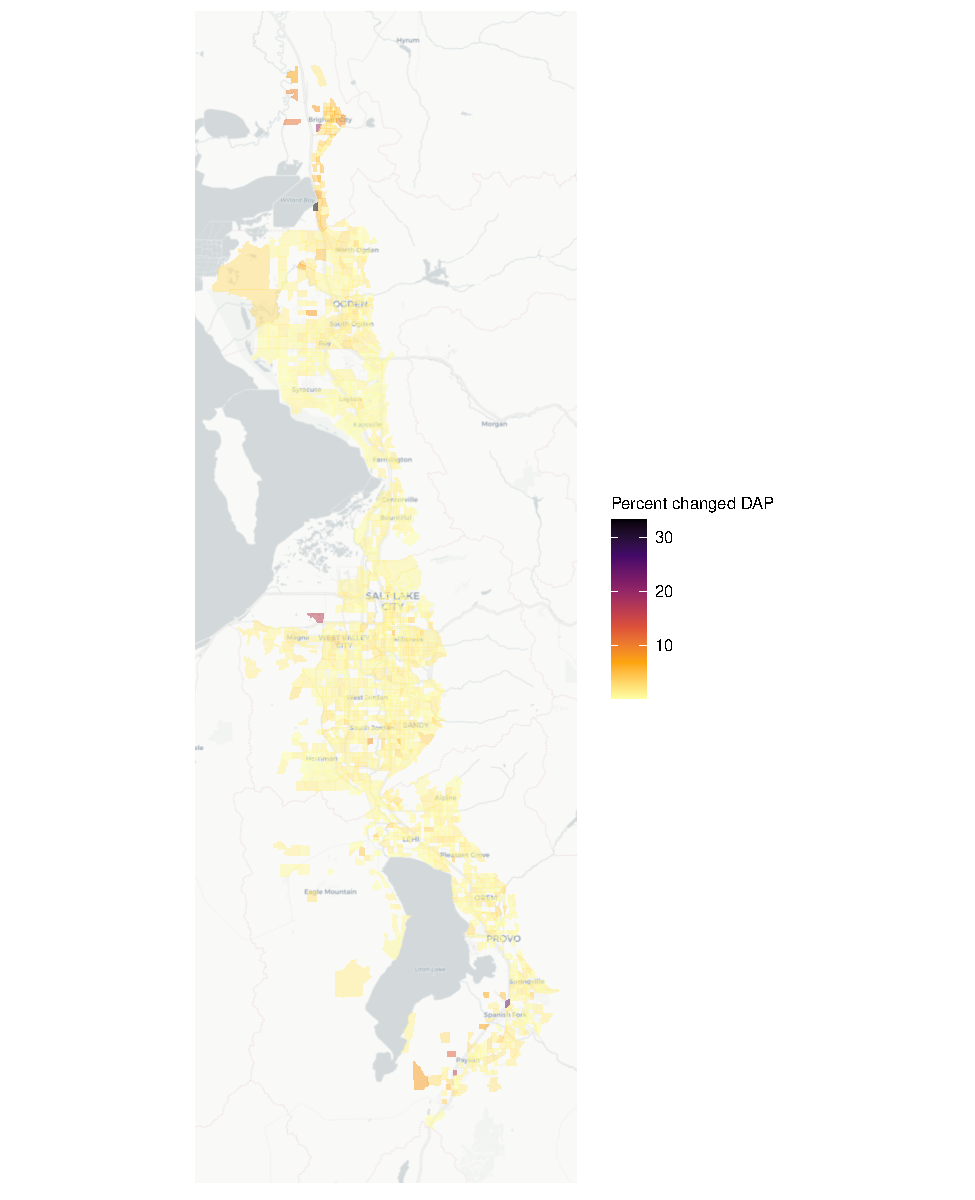
\includegraphics{wheelchair_cdap_files/figure-latex/dap-map-1.pdf}
\caption{\label{fig:dap-map}Percent of households with changed daily activity pattern between two scenarios.}
\end{figure}

In addition to these aggregate numbers, it is also worth considering where the
affected households are concentrated. Wheelchair use and disability in general
is not distributed evenly through the region. Figure \ref{fig:dap-map} shows the
concentration of households where at least one member changed its chosen
daily activity pattern between the scenarios by traffic analysis zone. Though
most areas of the region experience little if any alteration, some zones see as
many as 20 percent or 30 percent of their households change activity patterns.

\hypertarget{discussion}{%
\section{Discussion}\label{discussion}}

Disability status is almost never included in travel demand forecasting
efforts for a number of reasons. First is a practical issue; each element
of a population included in a model requires additional effort to not only catalog
and calibrate in the base year, it requires forecasting that variable out into
the future planning years. Limiting the variables considered to the typical set
of age, employment status, household size, and income (among potentially a few
others) reduces burden on planners and simplifies the data management pipeline.
Second, the variety of possible travel-limiting disabilities and the perceived
small size of the affected population might make understanding the travel
behavior impacts of all potential disabilities a high-cost, low-impact proposal
in the large scheme of a travel model.

There is an important philosophical argument to be had about the equity
implications of considering disability within travel forecasting efforts. On
one hand, excluding disability from travel behavior models might reinforce the
``invisibility'' of this population when developing transportation plans and other
public policies. If a population is not modeled, it is difficult to evaluate how
various policies would impact them within a model. Thus household income is left
as virtually the only equity consideration in travel forecasts \citep{bills2012}.
On the other hand, current
travel modeling practice assumes constant behavioral impacts into the future. Is
is correct or fair to assume that the travel costs and obstacles currently
faced by individuals with disabilities will continue unabated twenty or thirty
years from now? Many of these same philosophical questions also apply to
other variables that might be observed to affect travel behavior, such as race
or ethnic group or religious affiliation \citep[e.g.,][]{vyas2015}.

This study suggests that omitting wheelchair use is not without cost.
The impact of wheelchair use on individual travel behavior appears to be
substantial, and is potentially of a scale to affect travel forecasting results
in particular areas. Further research is required, but it is possible that wheelchair
use could result in different outcomes for transit ridership and local trip
production at least. The daily activity pattern model presented in this research
is only the first step in a typical travel activity modeling process. Future
research should undertake a rigorous evaluation of the effect of wheelchair use
on vehicle ownership, tour frequency, activity location choice, and travel mode.
It is possible that other disabilities will need to be investigated as well.

The NHTS provides a sufficiently large sample of individuals who use wheelchairs
to undertake the analysis presented here. It is unlikely, however, to be useful
for some of the other travel activity models just described. Activity location
choice models require substantially more precise geographic detail --- including
detail on non-chosen alternative locations --- than is provided in the NHTS.
Local household travel surveys are unlikely to sample enough individuals who use
wheelchairs to estimate robust effects without targeted oversampling techniques.
The results of this study raise a question as to whether planning agencies
ought to consider conducting this oversampling to enable future research.

The model specifications presented in Table \ref{tab:model-coef} each consider
wheelchair use independently from other variables. It is likely however, that there
could be some interaction effects among the various individual attributes.
To wit: do wheelchair users who hold bachelor's degrees behave differently
with respect to activity pattern than wheelchair users with less education?

This study used information from all United States metro areas between one and
three million in population. It is possible that the obstacles wheelchair users
face in some of these metro areas are larger or smaller than others. It is also
possible that larger or smaller metro areas would present different challenges
or provide different resources to wheelchair users. The same logic extends to other
countries besides the United States. Examining the role of wheelchair use on daily
activity pattern in other national contexts is important, as would be further
research on other categories of disability.

\hypertarget{conclusion}{%
\section{Conclusion}\label{conclusion}}

In the generation since the enactment of the ADA in 1990, much progress has
been made in the United States in making public accommodations and transportation
services available to all users regardless of their disability status.
Despite this progress, the results of this research suggest that wheelchair
users still face substantial friction in their daily travel after controlling
for age, income, and other common sociodemographic characteristics. Though
the size of the wheelchair-using population is relatively small --- particularly
within the context of a regional travel demand model --- it may be spatially
concentrated to the point where it could influence forecasts for individual transit
services or local highway facilities.

As transportation planners are being asked to consider equity in more policies
and contexts, the needs of wheelchair users and others with travel-limiting
disabilities should be considered in more contexts. The exclusion of wheelchair
users from travel models means that services and policies aimed at assisting
this community may be devalued relative to highway capacity and other more
traditional projects. The consequences of this exclusion should be investigated,
as well as the exclusion of other variables that would enable a more holistic
assessment of winners and losers in the transportation system.

\hypertarget{acks}{%
\section*{Acknowledgements}\label{acks}}
\addcontentsline{toc}{section}{Acknowledgements}

Figures and tables in this paper were created with a variety of R
packages \citep{R-ggplot2, R-modelsummary, R-ggspatial}. The authors would like to thank
Chris Day and Christian Hunter for their help in preparing this analysis.

This work was supported by the Utah Department of Transportation and the
Federal Transit Administration. The authors alone are responsible for the
preparation and conclusions presented herein. The contents do not necessarily
reflect the views, opinions, endorsements, or policies of the Utah Department of
Transportation of the US Department of Transportation. The Utah Department of
Transportation makes no representation or warranty of any kind, and assumes no
liability therefore.

\hypertarget{references}{%
\section*{References}\label{references}}
\addcontentsline{toc}{section}{References}

\bibliography{book.bib}


\end{document}
